\section{Hardware}
\label{sec:hardware}

This section provides instructions for maintaining all of the SuperDARN Radar's hardware. This includes the transceiver boxes, antennas and the server network.

\subsection{Antennas}
\label{subsec:hw_antennas}
The radar has 20 antennas altogether; 16 in the main array and 4 as part of the secondary array. Each antenna consists of two halves which, put together, makes a hexagon. It is the responsibility of the radar engineer to ensure that the antennas are always in good shape.

\subsubsection{Making antenna halves}
For making new antenna halves, use an existing example as reference. Some of the parts will also need to be scavenged from the broken element being replaced. \figref{hw_element} below shows the dimensions for the antenna element itself.

\begin{figure}[H]
	\centering
	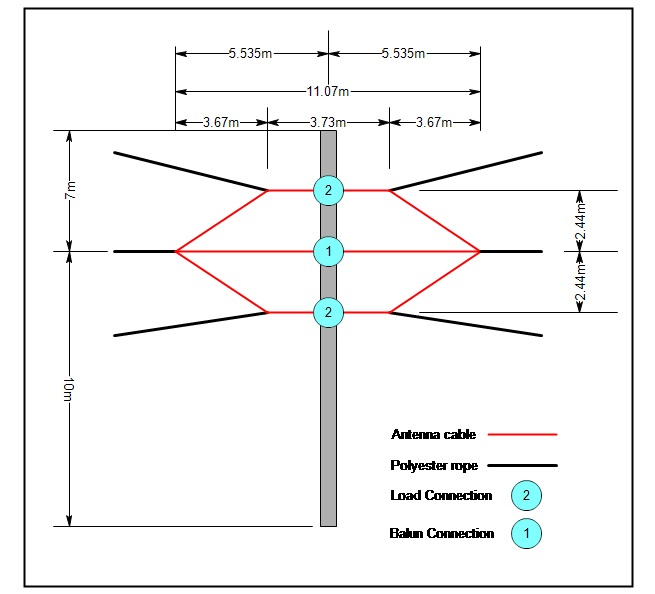
\includegraphics[width=0.7\textwidth]{images/hardware/element.jpg}
	\caption{Antenna element measurements.}
	\label{fig:hw_element}
\end{figure}

It is recommended that at least four already made antenna halves be kept in the radar hut. That way, spares can be made during takeover and simply replaced if any elements brake throughout the year.

\subsubsection{Measuring cable loss}
To test an antenna, the cable loss can be measured for each antenna from within the radar hut. To do this, the mobile antenna analyzer can be used. These values should be recorded and entered into the month-end reports.
\par
The antenna analyzer is usually kept in the radar hut for convenience. Measurements should be made at least every second month to ensure that all antennas are still in good condition. To make a cable loss measurement:
\begin{enumerate}
	\item Plug in the analyzer's power supply.
	\item Disconnect the antenna cable from the transceiver box.
	\item Connect the antenna cable to the port on the analyzer.
	\item Read and record the value shown for the range between 12.5 MHz and 14.5 MHz.
	\item Reconnect the antenna cable to the transceiver box.
\end{enumerate}
\par
There are several other measurements that can also be made with the analyzer, but none of which will provide any useful information for regular maintenance checks. However, they might be useful for fault finding with the antenna baluns or load connections.

\clearpage

\subsection{Transceiver Boxes}
\label{subsec:hw_boxes}

This section provides a guide for changing settings, servicing and troubleshooting a T3 radar transceiver box. The transceiver box should be laid out and wired according to diagram in \figref{hw_box_diagram}.
\par
Inspect the box and make sure that each PCB is in the correct position and that all wires are in place. Check the green Phoenix connectors for any loose wires and tighten the screws if necessary. Check that the boards are mounted properly to the aluminium plate, especially the power amplifier and tighten the screws, if necessary. Check that there is no loose debris inside the box e.g. small pieces of solder wire, which can cause a short.

\begin{figure}[H]
	\centering
	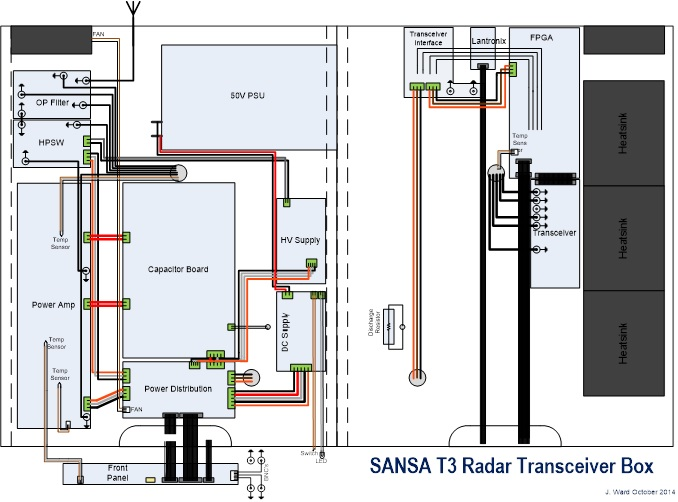
\includegraphics[width=0.7\textwidth]{images/hardware/box_diagram.jpg}
	\caption{T3 Transceiver box diagram.}
	\label{fig:hw_box_diagram}
\end{figure}

\subsubsection{Equipment Setup}

You will require the following equipment for setting up and testing the transceiver boxes:
\begin{itemize}
	\item 4-Channel Tektronix Scope (TDS 3054C).
	\item Tektronix current sensor module and current probe (TCPA300 + TCP312).
	\item Agilent 4-Channel Scope (MSO6104A)
	\item Radar Lab 2.0
	\item	AWG (33250A)
	\item	High voltage scope probe
	\item	DMM
	\item	50 Ohm dummy load
	\item	Bench power supply (60V, 10A)
	\item	SMA 50 Ohm terminator
\end{itemize}

\subsubsection{Preparing a Transceiver Box}

\begin{enumerate}
	\item Starting on the bottom side, remove all the green Phoenix connectors from their headers.
	\item Remove the chassis fan connector (P7) from the Power Distribution Board.
	\item Remove the ribbon cables (P2, P3 and P5) from the Front Panel.
\end{enumerate}

\begin{figure}[H]
	\centering
	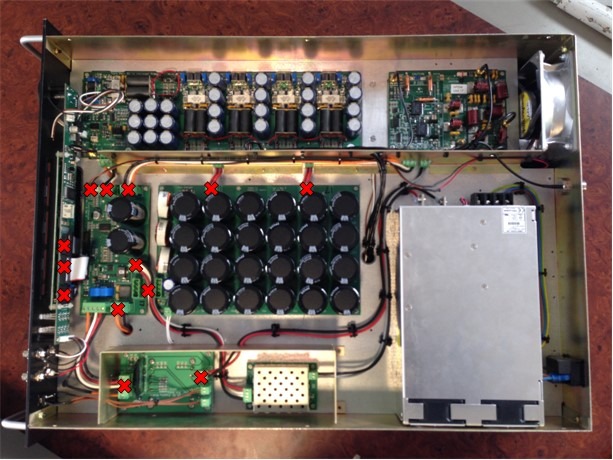
\includegraphics[width=0.7\textwidth]{images/hardware/box_prep.jpg}
	\caption{Preparing the transceiver box}
	\label{fig:hw_box_prep}
\end{figure}

\subsubsection{50V Power Supply}

\begin{enumerate}
	\item The C13 mains connector on the back of the box requires a 3.15A slow blow fuse. Check that the fuse is inserted and intact.
	\item Insert the AC mains power cord on the 50V PSU and switch it on. Use a DMM to check that the output voltage is 50V ±0.5V. If the voltage is out of tolerance then use a small screwdriver to adjust the small potentiometer (Vadj) on the back of the PSU itself.
	\item Power down.
\end{enumerate}

\begin{figure}[H]
	\centering
	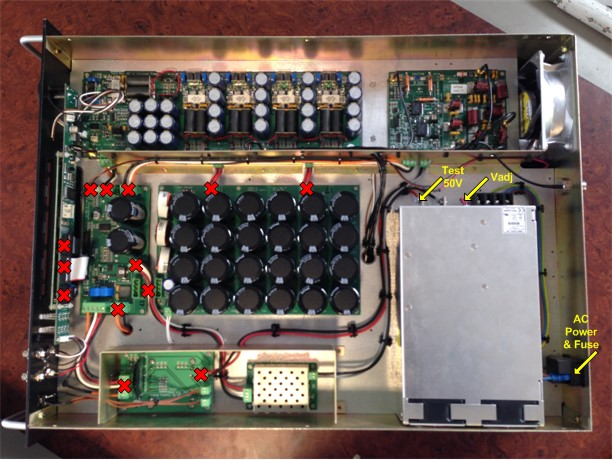
\includegraphics[width=0.7\textwidth]{images/hardware/box_50v.jpg}
	\caption{Testing the 50V power supply}
	\label{fig:hw_box_50v}
\end{figure}

\subsubsection{DC Supply}

\begin{enumerate}
	\item Connect J1 on the DC Supply Board (50V). Make sure J2 and J3 are also connected to the switch on the front plate and that the switch is in the \textbf{OFF} position. Leave all other connections for now. Switch the mains power on again.
	\item Check D11 and D12. They should both be \textbf{OFF}. Now toggle the switch on the front plate.
	\item Check that D12 lights \textbf{ON}. and that D11 stays \textbf{OFF}.
	\item If D2 does not light up, pull the connector J2. If it then lights up, there is a problem with the switch; check that the wires are secure in the switch connector and/or check the switch by doing a continuity test. Check that there is nothing connected to the DC Supply Board that could be pulling current, there may be a short circuit causing the module to shut-down.
	\item If that still does not solve the problem, the module has likely failed and should be replaced.
	\item If D2 lights ON, then the relay has probably failed and should be replaced.
	\item Finally check the output voltage on the 15V line of J4. It should be about 16.2V at no load. This is to compensate for the voltage drop in the thermistor, which is connected in series with the 15V line between J4 on the DC Supply Board and J6 on the Power Distribution Board. Check that the thermistor is working by measuring the 15V line on the Power Distribution Board side of the thermistor. At no load it should show that same voltage as measured earlier, about 16.2V.
	\item Disconnect the white wire (50\_en) from the Phoenix connector at J6 on the Power Distribution Board. Use the desktop power supply to apply exactly 3.3V to this wire. This will toggle the relay and light up D2. If this does not work, there is likely a problem with the relay and it should be replaced. Verify by measuring the voltage on the 50V line of J4 on the DC Supply Board. Replace 50\_en back into J6.
	\item Switch off the 15V on the front plate and the mains power too.
\end{enumerate}

\begin{figure}[H]
	\centering
	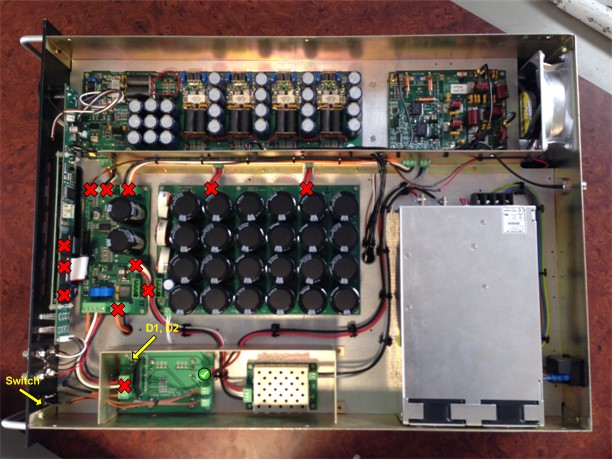
\includegraphics[width=0.7\textwidth]{images/hardware/box_dc.jpg}
	\caption{Testing the 15V DC-DC supply board}
	\label{fig:hw_box_dc}
\end{figure}

\subsubsection{Power Distribution}

\begin{enumerate}
	\item Insert the Phoenix connector into J6 on the Power Distribution Board. Insert the Special Test Cable (STC) into P2. Leave all other connections on the Power Distribution Board disconnected for now.
	\item For reference the pins required on the STC are:
		\begin{itemize}
			\item Pin 1 – Ground
			\item Pin 19 and 20 TxRx (switching signal for PA and HPSW)
			\item Pin 18 and 16 – 3.3V (50V enable, HV enable)
			\item Pin 3 – Ground
		\end{itemize}
	\item Switch on the mains power and then switch on the 15V power.
	\item Check D1 and D2 again on the DC Supply Board. If D1 does not light up or if D1 flashes then there is a fault on the Power Distribution Board. If this is the case, check that the thermistor is working as the inrush current to the capacitors C9 and C10 will trip the 15V supply if it is not limited by the thermistor. Otherwise you will have to fault find on the Power Distribution Board. The IC U2 and the 5V module are possible failure points as well as the regulators U1 and U3.
	\item If all goes well, D1, D2 and D3 on the Power Distribution Board should light up as well as D8.
	\item If D1 is off, check the 3.3V regulator U1; if D2 is off, check the 5V DC-DC converter; if D3 is off, the 15V line is faulty, so use the previous steps to debug. D8 is the fan controller, check U3.
	\item Measure voltages on P1, P3 and P8 (3.3V, 5V and 15V) using a DMM. 3.3V±0.1V; 5V±0.2V and 14.6V is nominal.
	\item Use 3.3V from the desktop power supply to turn on the relay via the STC and test the 50V on P9 (D4 should also light up when you do this).
	\item Switch off the 15V from the front switch, plug in the fan on header P7, and switch on again. The fan should start up. Adjust potentiometer R35 to control the fan speed. If the fan does not start up, you likely have an inrush current problem or U3 is faulty.
	\item If all is well, switch off from the front switch and move on to step 5.
\end{enumerate}

\begin{figure}[H]
	\centering
	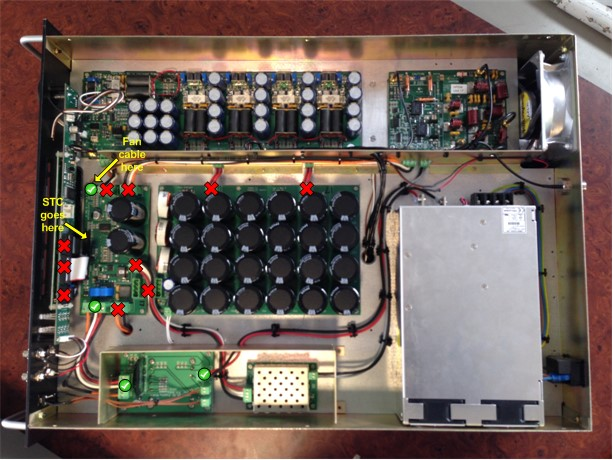
\includegraphics[width=0.7\textwidth]{images/hardware/box_distro.jpg}
	\caption{Testing the power distribution board}
	\label{fig:hw_box_distro}
\end{figure}

\subsubsection{Front Panel}

\begin{enumerate}
	\item Connect the ribbon cable P2 on the Front Panel to the Power Distribution Board. Power on.
	\item There are three LED’s on the Front Panel, indicating voltages 15V, 5V and 3.3V. If one of the LED’s is off check the 5V or 3.3V regulators on the Front Panel. The 15V comes from the Power Distribution Board so a fault on the 15V line by now will be caused by the Front Panel Board so fault find there.
	\item There is also one row of four LED’s on the front plate which should light up. The second row of LED’s should be off but may flash momentarily at switch on.
	\item Scroll using the turn knob to the voltage screen on the Front Panel and check that the voltages are displaying. The voltages from the FPGA will be blank at this time. If any other voltages from the Power Distribution Board are missing then check the ribbon cable. Remember to apply 3.3V to the relay to see the 50V display.
	\item Power off.
	\item Now connect the remaining ribbon cables P3 and P5. Power up and check for faults. If a fault occurs after this then the problem is either with the Lantronix Board or the FPGA. The likely cause is a damaged ribbon cable, so check that first before continuing to fault find.
	\item D1 on the Lantronix board should light up if all is OK.
	\item Power off.
\end{enumerate}

\begin{figure}[H]
	\centering
	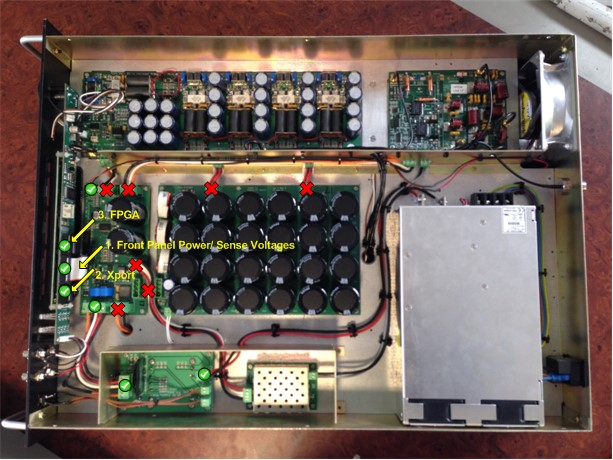
\includegraphics[width=0.7\textwidth]{images/hardware/box_fp.jpg}
	\caption{Testing the front panel board}
	\label{fig:hw_box_fp}
\end{figure}

\subsubsection{Capacitor Farm}

\begin{enumerate}
	\item Connect the Phoenix connector between the Power Distribution Board (J3) and the Capacitor Board (J1).  Make sure that the discharge resistor is connected at J2 on the Capacitor Board.
	\item Power on and apply the 3.3V signal to the STC. When 3.3V is applied the 50V will enable and D3 on the Capacitor Board will light up. Disconnect the 3.3V signal and D3 should start to dim. After approximately 15 to 20 seconds, D3 should be completely off.
	\item If the Capacitor Board does not discharge, check the MOSFET, Q2. Also check that the relay has shut off the 50V supply.
	\item Check that the Front Panel Board does not brown out and reset. If this happens, there is a problem with C9 and C10, they are not large enough or are not connected properly, check this with a continuity test.
\end{enumerate}

\begin{figure}[H]
	\centering
	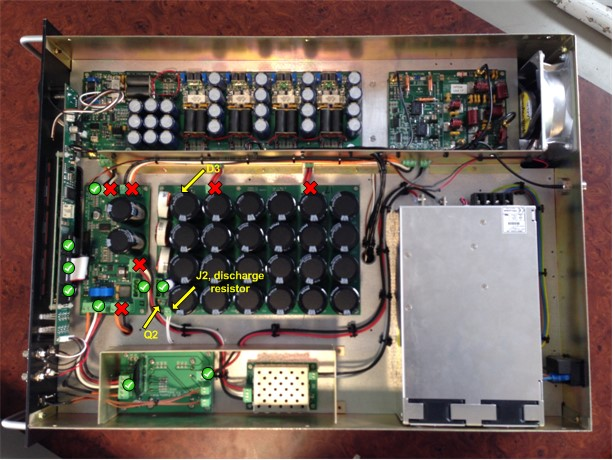
\includegraphics[width=0.7\textwidth]{images/hardware/box_cap.jpg}
	\caption{Testing the capacitor board}
	\label{fig:hw_box_cap}
\end{figure}

\subsubsection{High Power Switch}

\begin{enumerate}
	\item Switch on the AWG and set the frequency to 12.5 MHz and set the amplitude to 500mVp-p. Connect a BNC cable between the Output of the AWG and Channel 1 on the Agilent MSO6104A to view the waveform. Make sure to press ”Output” on the front face to enable the waveform. Remember to set the impedance of the channel to 50$\Omega$. Check that the waveform displayed is correct.
	\item Connect the Special Test Cable (STC) to the “Tx/Rx” of the Radar Lab 2.0 via the BNC-connector and insert the other end into P2 of the Power Distribution Board. This will give us manual control over some of the FPGA functions needed for the tuning process.
	\item For reference the pins required on the ribbon cable are:
		\begin{itemize}
			\item Pin 1 – Ground
			\item Pin 19 and 20 Tx/Rx (switching signal for PA and HPSW)
			\item Pin 18 and 16 – 3.3V (50V enable, HV enable)
			\item Pin 3 – Ground
		\end{itemize}
	\item Terminate the output at the antenna port with the 100W dummy load.
	\item Make sure that the Phoenix connector J2 is removed from the HPSW. Replace it with a connection to the bench PSU. Set the PSU to 30V and limit the current to 1A.
	\item Switch on the power of the transceiver box, the Radar Lab 2.0; as well as the 30V from the PSU to the HPSW.
	\item Check that the Tx/Rx pulses are coming through on P5.
	\item Check the TP\_A is a replica of the Tx/Rx signal. If there is no waveform on TP\_A, check that the CPLD is programmed. Otherwise, there is possibly a fault with the CPLD or its clock.
	\item Check that P6 switch waveform goes from a DC off-set of about half of the 15V supply (7.5V) up to the HV supply voltage, which in this instance is set to 30V.
	\item Power off.
	\item Replace the 30V with the 1000V (reconnect the phoenix connector from the HV supply board). Switch on and check that P6 is now the switched 1000V.
	\item Power off and return to 30V supply.
		\begin{figure}[H]
			\centering
			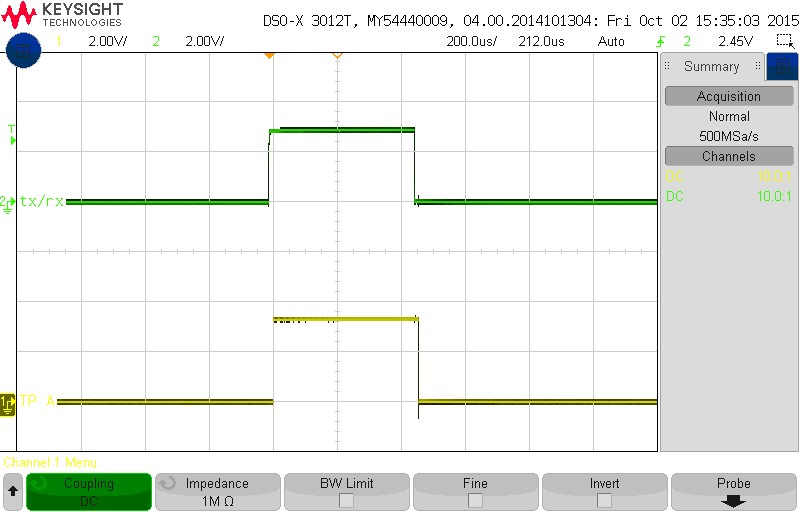
\includegraphics[width=0.45\textwidth]{images/hardware/signal_1.jpg}
			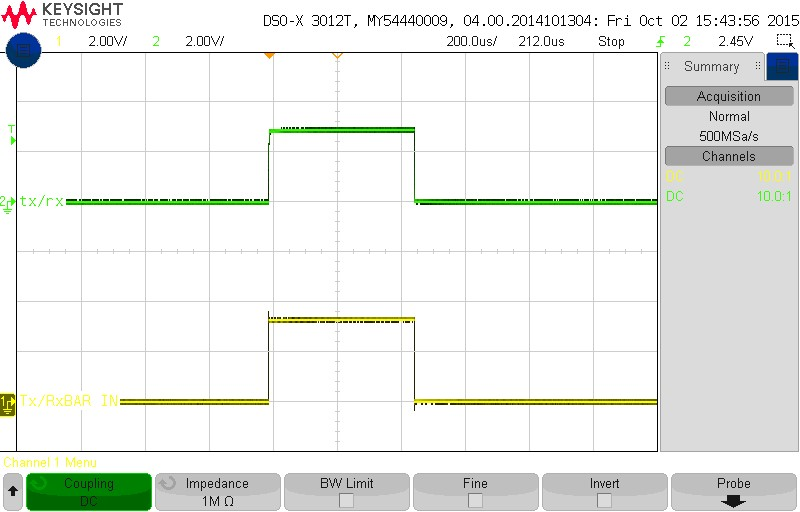
\includegraphics[width=0.45\textwidth]{images/hardware/signal_2.jpg}
			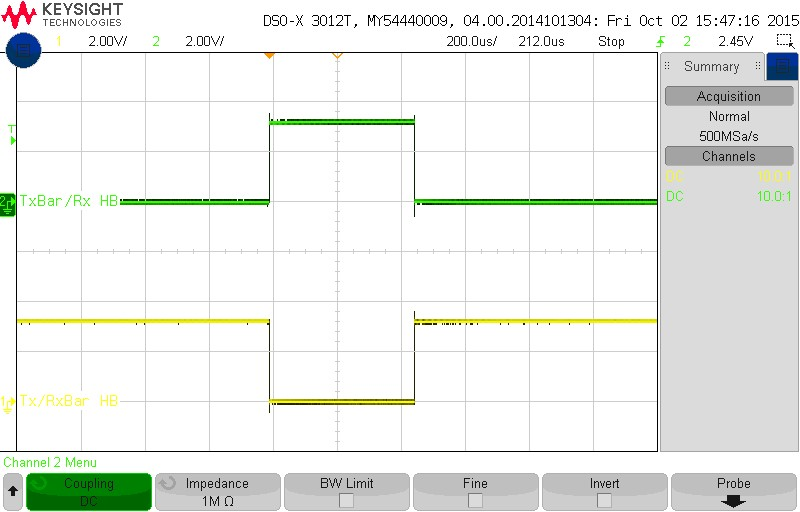
\includegraphics[width=0.45\textwidth]{images/hardware/signal_3.jpg}
			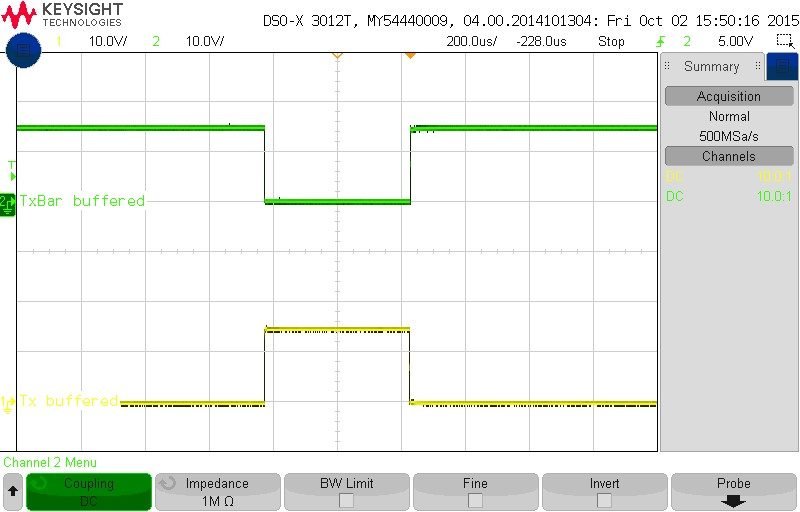
\includegraphics[width=0.45\textwidth]{images/hardware/signal_4.jpg}
			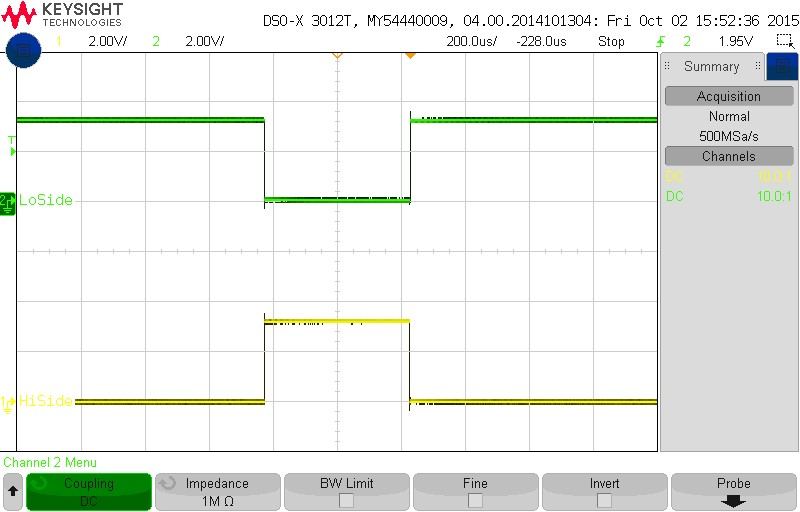
\includegraphics[width=0.45\textwidth]{images/hardware/signal_5.jpg}
			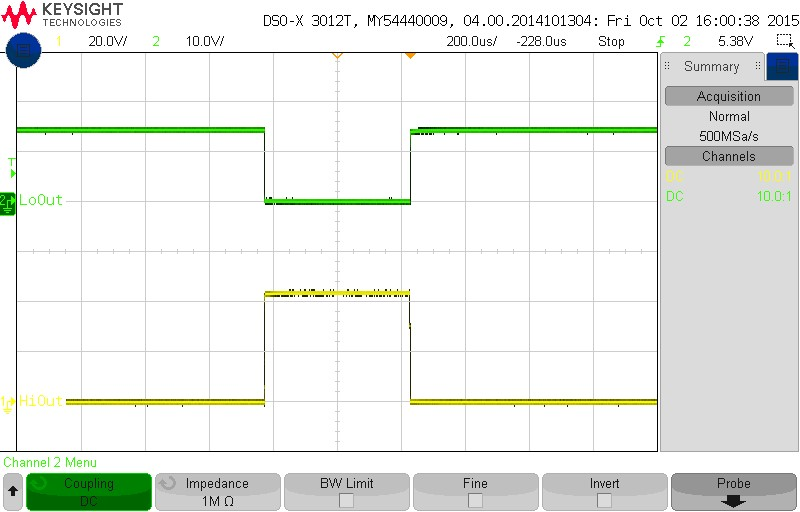
\includegraphics[width=0.45\textwidth]{images/hardware/signal_6.jpg}
			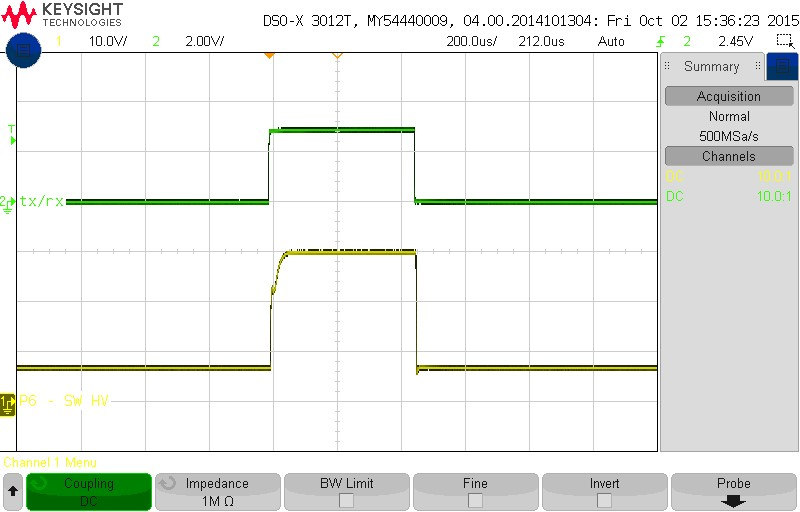
\includegraphics[width=0.45\textwidth]{images/hardware/signal_7.jpg}
			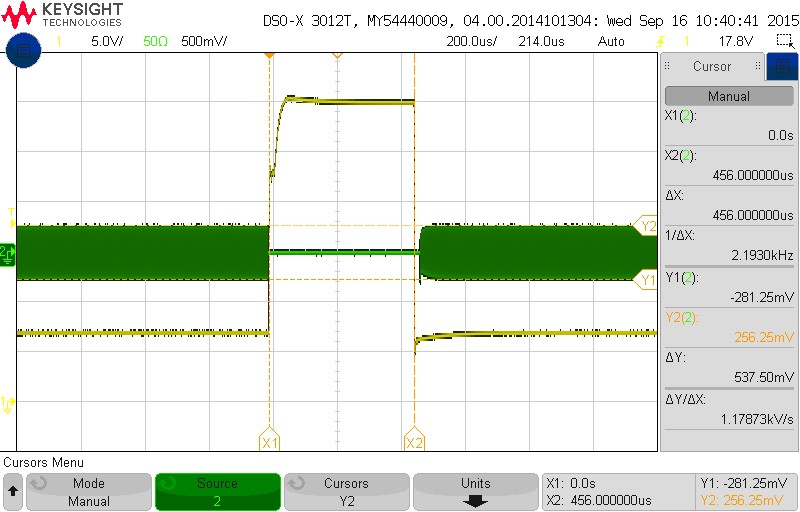
\includegraphics[width=0.45\textwidth]{images/hardware/signal_8.jpg}
			\caption{First HPSW oscilloscope measurements.}
			\label{fig:hw_hpsw_signals_1}
		\end{figure}
	\item Remove the dummy load and connect the RF signal to the antenna port (12.5 MHz frequency and 0 dBm amplitude).
	\item Make sure that you terminate the input port from the power amp or leave it connected to the power amp.
	\item Power on.
	\item Check that the signal from the antenna can be seen at the receive port, when the Tx/Rx switches low. You can also check that there is no leakage into the input port by terminating the receiver port and measuring on the input.
		\begin{figure}[H]
			\centering
			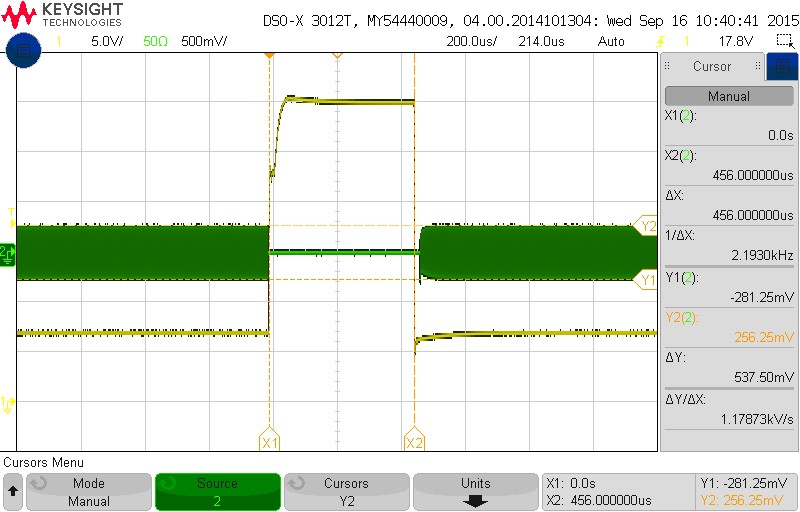
\includegraphics[width=0.45\textwidth]{images/hardware/signal_9.jpg}
			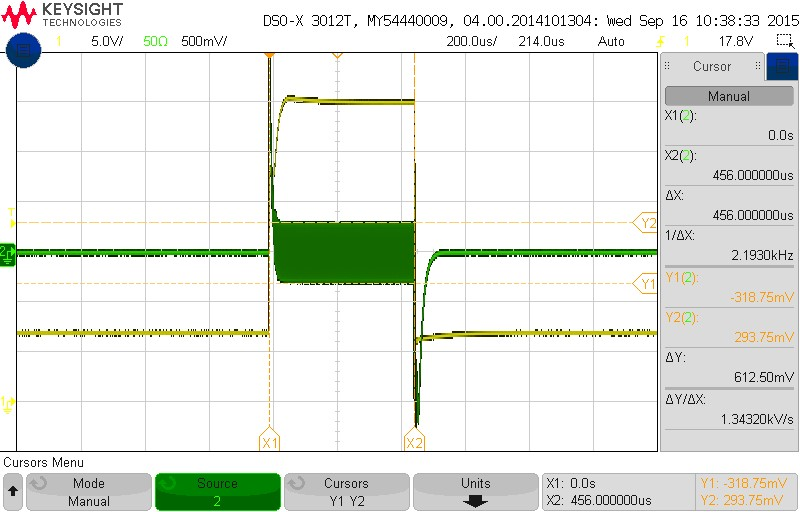
\includegraphics[width=0.45\textwidth]{images/hardware/signal_10.jpg}
			\caption{Second HPSW oscilloscope measurements.}
			\label{fig:hw_hpsw_signals_2}
		\end{figure}
	\item Power off.
	\item Terminate the receiver port.
	\item Connect the RF signal to the input.
	\item Power on.
	\item Measure that the signal is getting through to the antenna port when the Tx/Rx signal is high. Also check that there is no leakage to the receiver by terminating the antenna port and measuring on the receiver port.
		\begin{figure}[H]
			\centering
			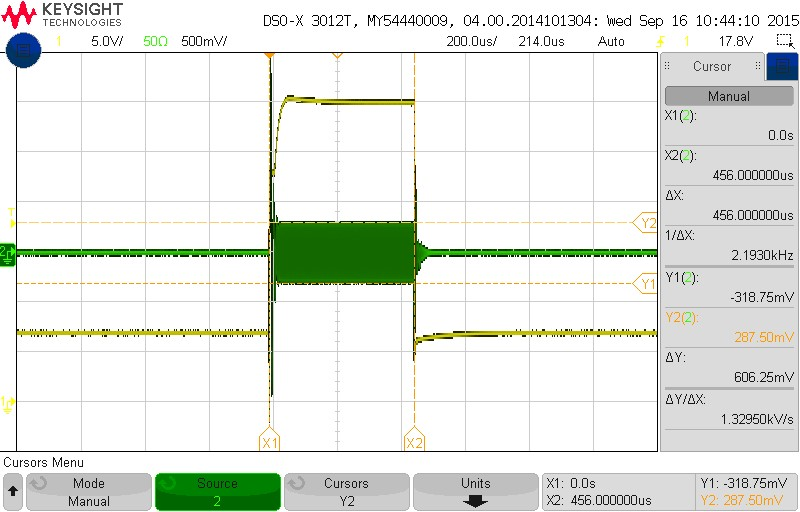
\includegraphics[width=0.45\textwidth]{images/hardware/signal_11.jpg}
			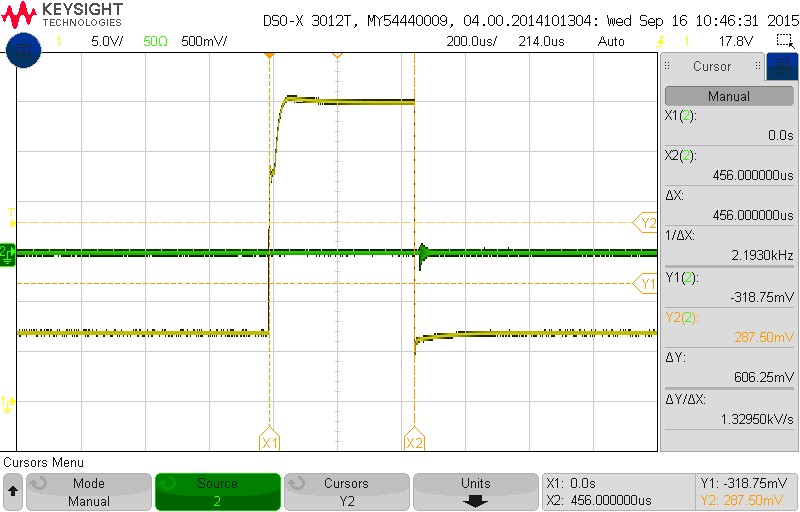
\includegraphics[width=0.45\textwidth]{images/hardware/signal_12.jpg}
			\caption{Third HPSW oscilloscope measurements.}
			\label{fig:hw_hpsw_signals_3}
		\end{figure}
\end{enumerate}

Once you are comfortable with what needs to be terminated when, where and why you can also use this shortcut testing sequence:
\begin{enumerate}
	\item Make sure that the Phoenix connector J2 is removed from the HPSW. Replace it with a connection to the bench PSU. Set the PSU to 30V and limit the current to 1A.
	\item Connect the Rx and PWRAMP RF connectors each to a channel on the oscilloscope (Channel 2 \& 3).
	\item Remove the dummy load and connect the RF signal to the antenna port (12.5 MHz frequency and 0 dBm amplitude)
	\item Power up the transceiver box mains, then the front panel and then the 30 V PSU supply.
	\item Check the outputs at P5, P6 and TP\_A (As described above).
	\item Now switch on the AWG output.
	\item Monitor the Rx and Tx signals on channel 2 \& 3; make sure that both the channels are set to a 200mV scale on the oscilloscope and they should have more or less the same pk-pk voltages. If Rx is more than 75 mV less than Tx; the problem is most probably with a faulty limiter (D4). Test it and if needed replace it. Other regular known culprits to be investigated (if it is found not to be the limiter) are Q3 and Q4 mosfets, located at the bottom of the HPSW board.
	\item Switch off the output of the AWG; switch off the 30 V PSU supply; switch off the front panel; and then lastly switch off the transceiver box mains.
	\item Remove the RF signal and connect the dummy load to the antenna port.
	\item Remove the oscilloscope channel connectors from the Rx and PWRAMP RF connectors and plug all the normal RF circuit connections back in.
	\item Replace the 30 V PSU supply with the 1000V (reconnect the phoenix connector from the HV supply board).
	\item Switch on the transceiver box mains; switch on the front panel and then switch on the 3.3 V supply connected to the STC.
	\item Check that P6 is now the switched 1000V (REMEMBER to use the HV oscilloscope probe when measuring voltages fed from the HV Supply!) Switch everything off in reverse order of step 12.
\end{enumerate}

\subsubsection{Power Amplifier}

\begin{enumerate}
	\item Connect the Tx Env output of the Radar Lab 2.0 to the ‘pulse’ modulation input on the back of the AWG/signal generator(Modulation In) to generate the RF pulses.
	\item Connect the Tx/Rx signal from the Radar Lab to the STC in the FGPA header on the Power Distribution Board.
	\item Connect 3.3V from the bench PSU to the 50V enable and the HV supply enable to the FPGA header on the Power Distribution board (via the STC). – This step should already be done!
	\item Remove the 50V supply leads from the capacitor board and replace with 30V from the bench PSU. Limit the current initially to 1A.
	\item Switch on Radar Lab 2.0
	\item Turn all potentiometers anti-clockwise all the way so that there is no bias on the gates of the MOSFETS.\\
(*** SHORTCUT: This step can be skipped.
If this is not a brand new power amp you can leave the potentiometers where they are, as to save time when setting the bias point of the VRF MOSFETS, in later steps. However in the case of the replacement of a power amp, when dealing with a brand new power amp board, note that the potentiometers are most probably turned all the way anti-clockwise already so that there is no bias on the gates of the MOSFETS.)
	\item Perform the ‘auto-balance’ function of the current probe. (PS Ensure that the probe is in a closed/locked state! Output of the scope on the TxRx channel should also be set to 1M$\Omega$)
		\begin{figure}[H]
			\centering
			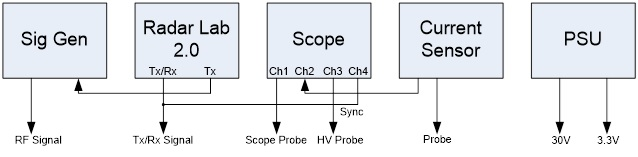
\includegraphics[width=0.7\textwidth]{images/hardware/amp_setup.jpg}
			\caption{Power Amplifier test station setup.}
			\label{fig:hw_amp_setup}
		\end{figure}
	\item Disconnect the HPSW from the Power Amp and terminate the output of the Power Amp (RF\_OUT RF connector). with the dummy load.
	\item Switch on the transceiver box (mains) and Front Panel switch (15V) – NOT YET THE 30 V PSU SUPPLY!
	\item Check that the Tx/Rx signal is present on P1.
	\item Check that P12 is around 9.8V using the DMM.
	\item Remove the thermistor from P14 and P12 should increase by about 20mV. The shows that the thermal compensation is working. Plug the thermistor back in.
	\item Check that P10 is a switched version of P1.
	\item Check that J3 (the square hole connection) should be the inverse of P10.
		\begin{figure}[H]
			\centering
			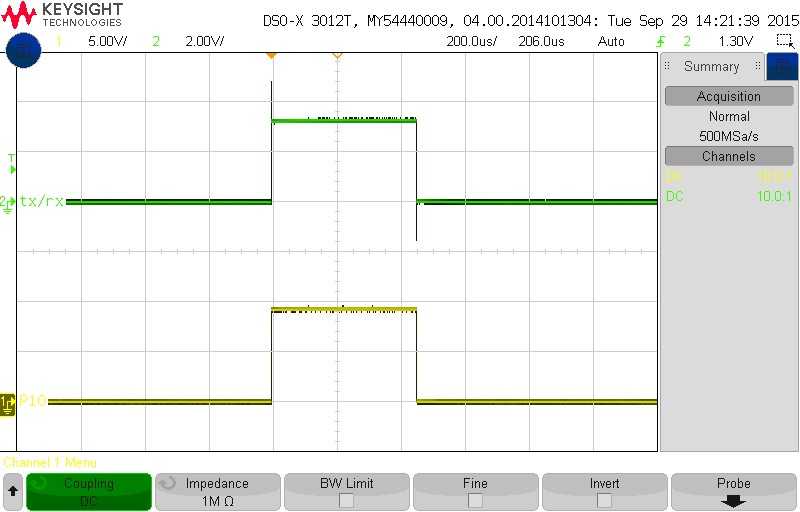
\includegraphics[width=0.45\textwidth]{images/hardware/signal_13.jpg}
			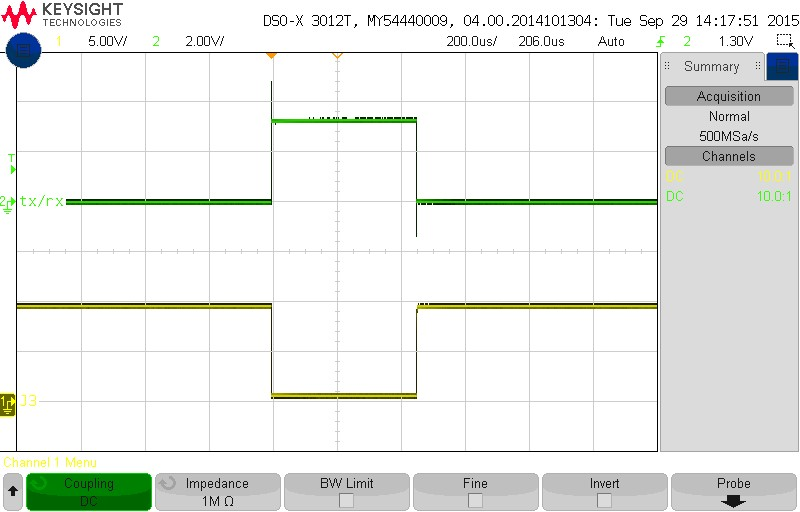
\includegraphics[width=0.45\textwidth]{images/hardware/signal_14.jpg}
			\caption{P10 should be a switched 9.8V signal and J3 should be the inverse of P10.}
			\label{fig:hw_amp_signals_1}
		\end{figure}
	\item Check that Pin 5 of Q1 is a switched 12V signal. This powers the HELA10. Also check that J5 (pin1) is the inverse of Pin 5 of Q1.
		\begin{figure}[H]
			\centering
			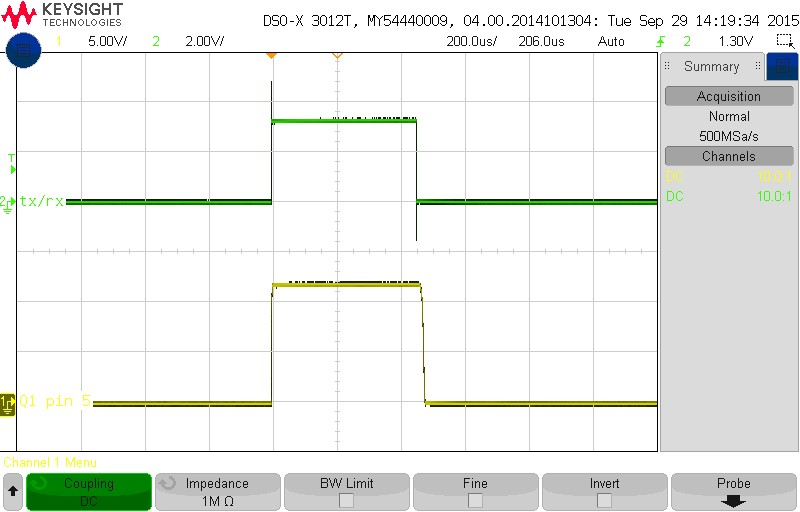
\includegraphics[width=0.45\textwidth]{images/hardware/signal_15.jpg}
			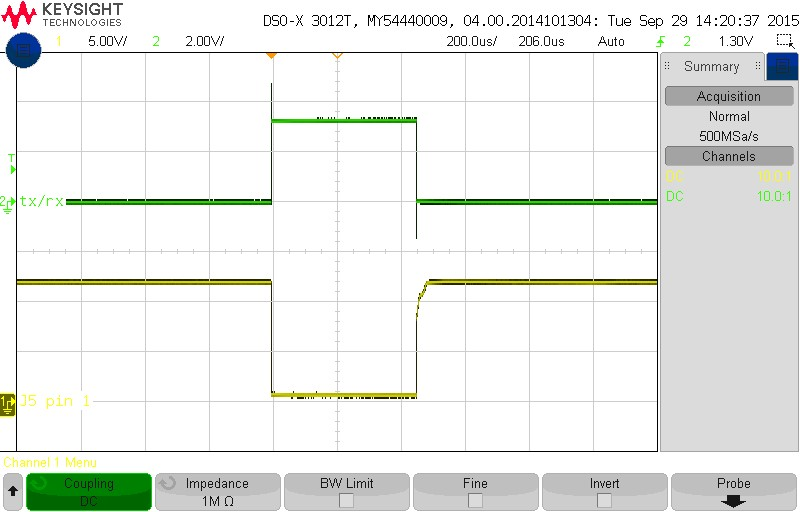
\includegraphics[width=0.45\textwidth]{images/hardware/signal_16.jpg}
			\caption{Switched 12V to power the HELA10 and J5 should be the inverse of Q1 (pin5).}
			\label{fig:hw_amp_signals_2}
		\end{figure}
	\item (Only applicable for brand new power amp boards.) Check that all the gates on the MOSFETS are at 0V. If not, check that the potentiometers are completely turned down.
	\item (Only applicable for brand new power amp boards.) Note: the gates are pre-biased using the potentiometers, onto which the drive pulse is added. This makes switching everything faster.
	\item (Only applicable for brand new power amp boards.) VRF MOSFETS pre-bias around 3.5V while the MRF MOSFETS pre-bias around 3V. The VRF part is better as it has more gain and a higher breakdown.
	\item Switch the 30V supply on.
	\item Attach the current probe to the copper wire bridge on the drain leads. Attach the scope probe to the corresponding test point on the MOSFET’s gate. Turn the potentiometer clockwise until you get close to the pre-bias point (3.5V). At this stage the current in the drain will start to rise when the Tx/Rx signal is high. Keep adjusting until the current pulse level is 200mA in the centre. The current pulse will at first be asymmetrical because there are two MOSFETS (adjust the first one to 100mA). Adjust the second MOSFETS gate voltage and monitor the current until you get 200mA current pulses its drain. Go back to the first drain and re-adjust to 200mA, if necessary.\\
(*** Make sure that the scope probe measuring the pre-bias point (Voltage – “Yellow”) is set to 1MΩ and that the oscilloscope triggers on this channel. Also make sure that the scope probe measuring the current pulse level (Amps – “Blue”) is set to 1 M$\Omega$ as well.)
	\item Repeat the above step for all 5 pairs.
	\item At this stage the current should read about 350mA @ 30V (410mA @ 50V).
	\item Switch off the 30V supply.
	\item Now connect the RF signal to the input (RF\_IN on the power amp board) with an amplitude of -20 dBm and a frequency of 12.5 MHz.
	\item Slowly increase the RF power up to 4 dBm.
	\item RF (TP\_IN) should be around 1V pk-pk; the output of the HELA10 (C12 and C14) should be around 2V pk-pk each and balanced; the input of the MOSFETS (“G” - Gate) should be about 750mV pk-pk. This tells us that the HELA10 is working.\\
(*** NOTE: At an amplitude of -20 dBm you don’t see anything on the oscilloscope immediately. Just start increasing the amplitude slowly whilst carefully monitoring it, until the RF signal is observed as described above.)
		\begin{figure}[H]
			\centering
			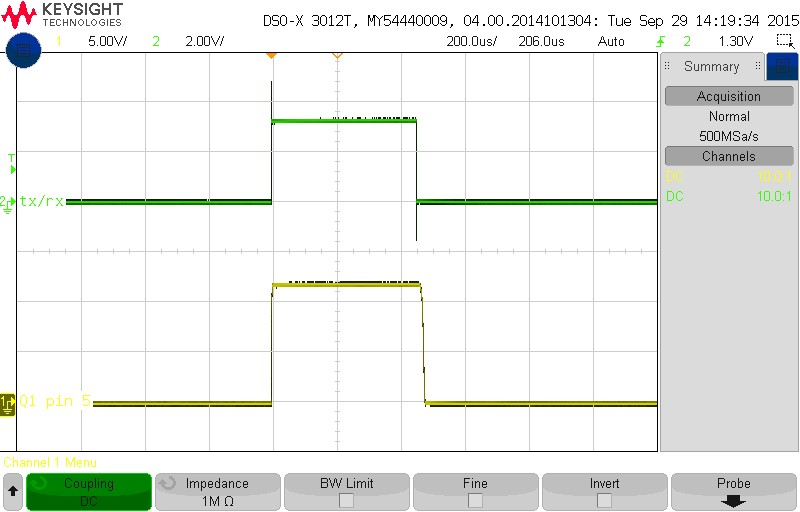
\includegraphics[width=0.45\textwidth]{images/hardware/signal_15.jpg}
			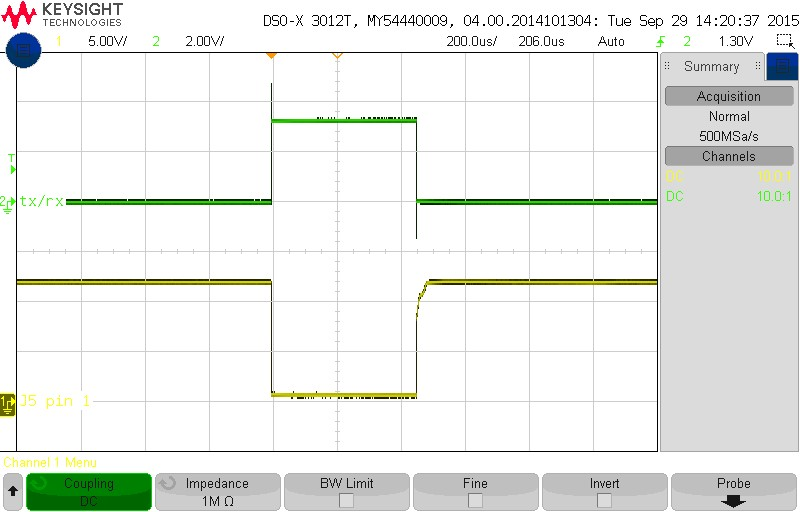
\includegraphics[width=0.45\textwidth]{images/hardware/signal_16.jpg}
			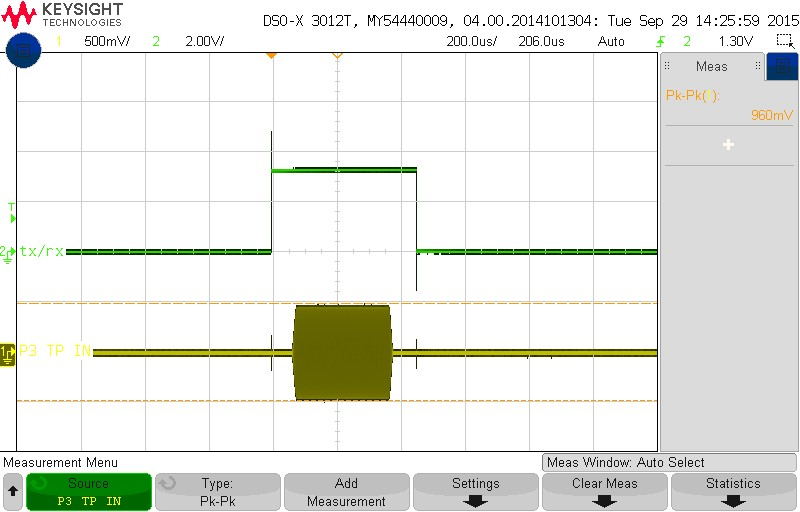
\includegraphics[width=0.45\textwidth]{images/hardware/signal_17.jpg}
			\caption{Input RF signal (P3) at 4 dBm is roughly 1Vp-p, the voltage at the outputs of the HELA10 should be about 2Vp-p and the voltage at the gate of the driver amp MOSFET should be 750mVp-p}
			\label{fig:hw_amp_signals_3}
		\end{figure}
	\item Turn the RF power back down to -20dBm. - IMPORTANT!
	\item Turn the 30V on again.
	\item Measure the output voltage at the Power Amp output (P20 – TP\_OUT). It should read around 11V pk-pk.
		\begin{figure}[H]
			\centering
			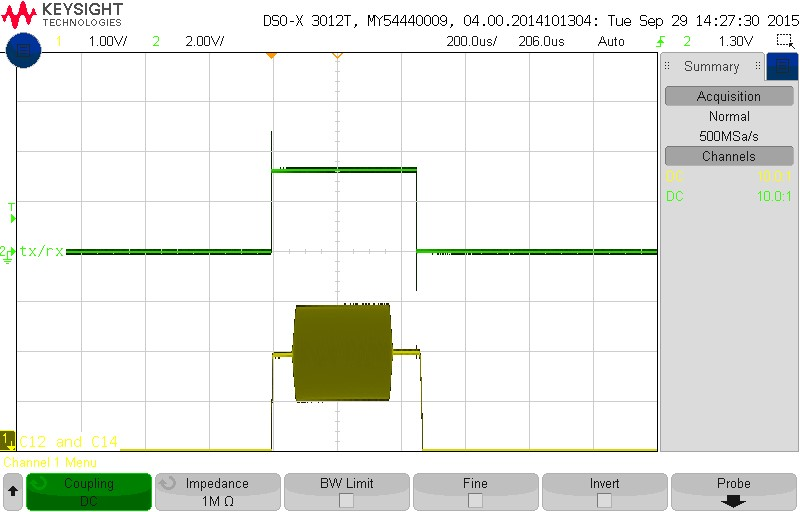
\includegraphics[width=0.45\textwidth]{images/hardware/signal_18.jpg}
			\caption{When the input is -20 dBm the output (P20) reads 11Vp-p.}
			\label{fig:hw_amp_signals_4}
		\end{figure}
	\item Slowly increase the input power. Carefully monitoring the output voltage. You will need to increase the current limiting on the PSU. At 0dBm you should see about 130V pk-pk. Keep increasing until you reach 600V pk-pk, this should be at an amplitude of about 7 dBms.
		\begin{figure}[H]
			\centering
			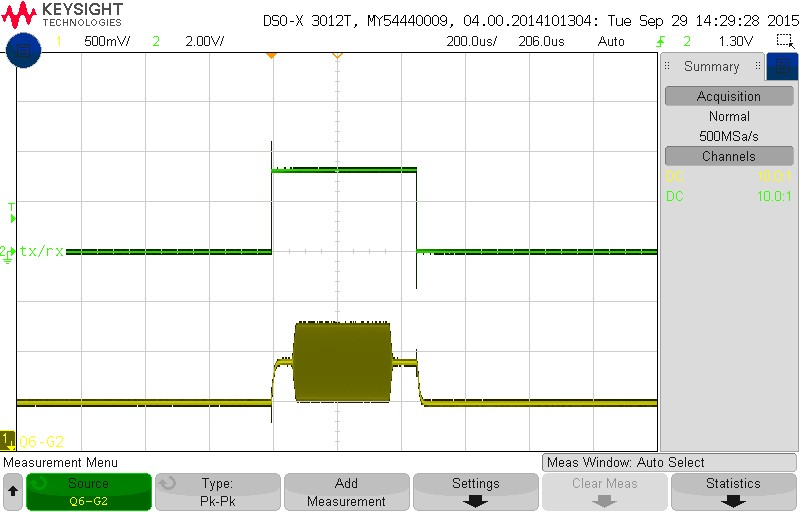
\includegraphics[width=0.45\textwidth]{images/hardware/signal_19.jpg}
			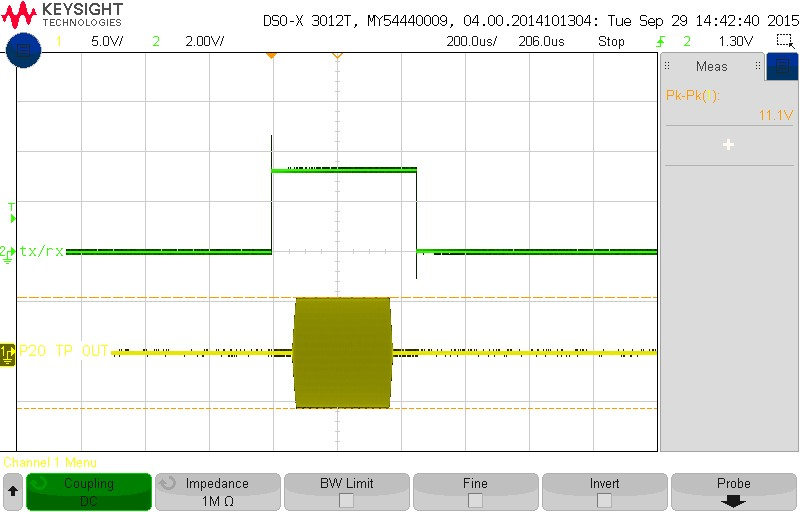
\includegraphics[width=0.45\textwidth]{images/hardware/signal_20.jpg}
			\caption{When the input is 0 dBm the output (P20) reads 130Vp-p. The output starts to saturate with an input signal of about 14dBm the output reads 600Vp-p.}
			\label{fig:hw_amp_signals_5}
		\end{figure}
	\item Now look at the drain voltages for each MOSFET. It should be somewhat symmetrical but the positive side will ramp up higher and there could be some slight ringing. Check the 3R3 damping resistors, if there is significant ringing.
		\begin{figure}[H]
			\centering
			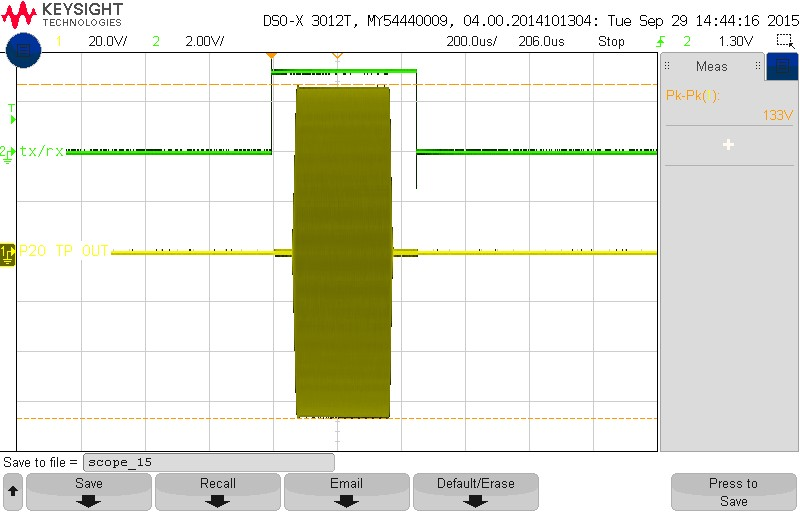
\includegraphics[width=0.45\textwidth]{images/hardware/signal_21.jpg}
			\caption{Drain voltage at 30V supply at 600Vp-p output. Check that there is not significant ringing on the drains of the MOSFET's and that the voltage does not exceed 170V.}
			\label{fig:hw_amp_signals_6}
		\end{figure}
	\item Turn the RF power back down to -20dBm. - IMPORTANT!
	\item If everything is okay then power off.
	\item Replace the 30V supply with the 50V supply (from the capacitor board) and repeat the above process, starting from -20dBm again and increasing to 950V pk-pk (This should be observed at an amplitude of more or less 13 dBms). Re-check all the drain voltages. We do not want to exceed 170V for the VRF’s. A typical value will be around 120V at 950V pk-pk output. (If a drain voltage exceeds these values; the corresponding VRF Mosfet should be checked and most likely be replaced.)\\
(*** ALTERNATE STEP 32 (including the HPSW and filter in the RF path): Un-terminate RF\_OUT, terminate Rx on the HPSW and reconnect the HPSW and Filter to the power amp. Connect the 100 W dummy load to the antenna port and measure the output at the output pin of the filter board. Replace the 30V supply with the 50V supply (from the capacitor board) and repeat the above process, starting from -20dBm again and increasing to 950V pk-pk (This should be observed at an amplitude of more or less 13 dBms). Re-check all the drain voltages. We do not want to exceed 170V for the VRF’s. A typical value will be around 120V at 950V pk-pk output. (If a drain voltage exceeds these values; the corresponding VRF Mosfet should be checked and most likely be replaced.))
	\item Turn the RF power back down to -20dBm. - IMPORTANT!
	\item Power down everything in the correct sequence.
		\begin{figure}[H]
			\centering
			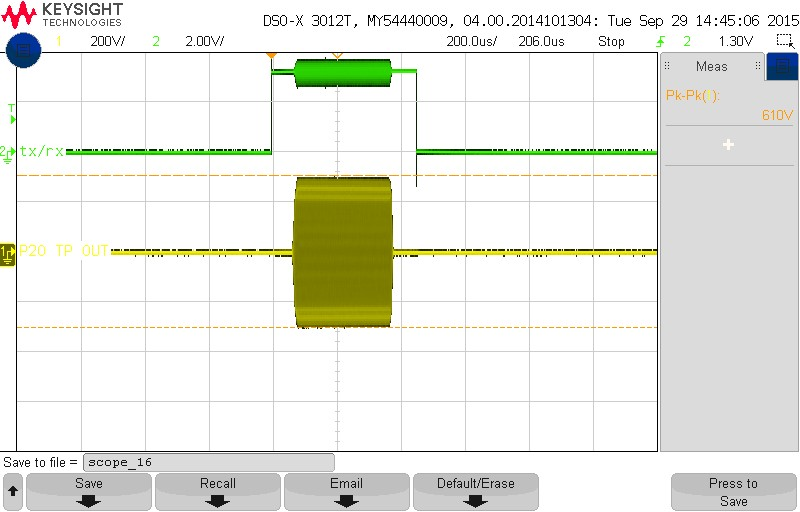
\includegraphics[width=0.45\textwidth]{images/hardware/signal_22.jpg}
			\caption{Drain voltage at 50V supply at 900Vp-p output.}
			\label{fig:hw_amp_signals_7}
		\end{figure}
\end{enumerate}

\subsubsection{FPGA}

\begin{enumerate}
	\item Connect  Phoenix connector J4 to the Power Distribution Board.
	\item This will provide power to the FPGA board and the RF Transceiver Board. Re-check that the voltages are at 5V and 15V before proceeding.
	\item The FPGA Board has its own power regulation for all the different supply voltages it requires. The easiest way to check that these are all in order is to look on the Voltage Screen on the Front Panel. You can also check LED’s D9, D10, D11, D12 and D13. Fault finding will be difficult but try and check the DC-DC converter modules, if there is a problem with one of the voltages. For example 1.8V is mostly limited to the 1GIG Ethernet controller, so check there if there is an issue with 1.8V (this fault has happened before).
\end{enumerate}

\begin{figure}[H]
	\centering
	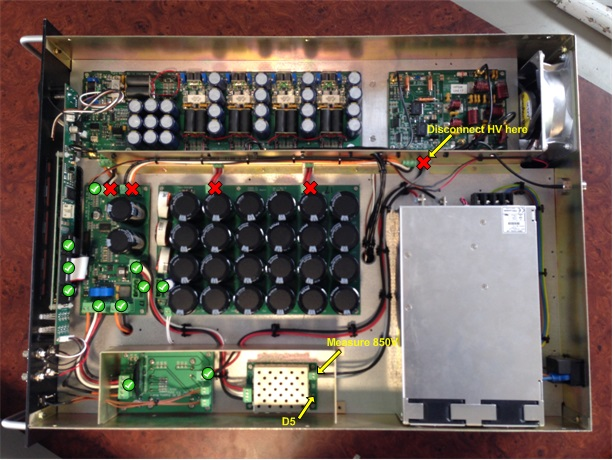
\includegraphics[width=0.7\textwidth]{images/hardware/box_fpga_txrx.jpg}
	\caption{Testing of FPGA and transceiver baord.}
	\label{fig:hw_box_txrx}
\end{figure}

\subsubsection{RF Transceiver}

\begin{enumerate}
	\item Connect the transceiver test board to the transceiver board and power it with 15 V from a test bench power supply.
	\item Verify that all 4 LEDs in the PWR LED bank on the transceiver test board are on.
	\item Verify that test pin P20 is at 10.5 V and P19 at 3.3 V on the transceiver board.
	\item Flip all of the switches on the transceiver test board on, one by one and verify that their corresponding LEDs respond accordingly (switch on and off when the switches are flipped).
	\item Switch on the AWG and set the frequency to 12.5 MHz and set the amplitude to 100mVp-p. Connect a BNC cable between the Output of the AWG and Channel 1 on the Agilent MSO6104A to view the waveform. Make sure to press “Output” on the front face to enable the waveform. Remember to set the impedance of the channel to 50$\Omega$ and use a 50$\Omega$ feed through connection on the oscilloscope channel being used. Check that the waveform displayed is correct.
	\item Connect the output of the AWG to the DAC2 port on the transceiver test board and Channel 1 on the Agilent MSO6104A to the DAC2\_Out port on the transceiver board.
	\item Verify that the signal observed is the same 12.5 MHz, 100mVp-p signal with possible minor amplitude losses (\~ 3 mV).
	\item Connect the output of the AWG to the DAC1(Tx) port on the transceiver test board and Channel 1 on the Agilent MSO6104A to the TxOUT port on the transceiver board.
	\item Verify that the signal observed is a 12.5 MHz, 25mVp-p signal. This is due to the Tx attenuator being set to maximum attenuation by default.
	\item Switch the LE (Latch Enable) of the Tx AGC bank on the transceiver test board on. This sets the Tx attenuator to minimum attenuation.
	\item Verify that the signal observed is a 12.5 MHz, 1Vp-p signal (800mV \~ 1V pk-pk).
	\item Switch through the attenuation switches in the Tx AGC bank on the transceiver test board one by one, starting at 1 dB all the way through to 16 dB. Verify after flipping each switch that the signal’s pk-pk amplitude decreases more and more with an increasing value of attenuation.
	\item Flip all the switches on the transceiver test board back to their original state (off).
	\item Connect the output of the AWG to the Antenna port on the transceiver board and Channel 1 on the Agilent MSO6104A to the MON2 port on the transceiver test board.
	\item Verify that the signal observed is the same 12.5 MHz, 100mVp-p signal with possible minor amplitude losses (\~ 3 mV).
	\item Connect the output of the AWG to the Current port and terminate the Pwr\_Amp port on the transceiver board and connect Channel 1 on the Agilent MSO6104A to the MON1 port on the transceiver test board.
	\item Verify that the signal observed is a 12.5 MHz, 70mVp-p signal with possible minor amplitude losses (\~ 3 mV).
	\item Switch SWB on, on the transceiver test board.
	\item Verify that the signal observed is a 12.5 MHz, 50mVp-p signal with possible minor amplitude losses (\~ 3 mV).
	\item Switch the power off.
	\item Connect the output of the AWG to the Pwr\_Amp port and terminate the Current port on the transceiver board and connect Channel 1 on the Agilent MSO6104A to the MON1 port on the transceiver test board.
	\item Switch the power on.
	\item Verify that the signal observed is a 12.5 MHz, 50mVp-p signal with possible minor amplitude losses (\~ 3 mV).
	\item Switch SWB off, on the transceiver test board.
	\item Verify that no signal is measured at the MON1 output port.
	\item Change the amplitude on the AWG to 1mVp-p as the amplification on the Rx signal path is very large and one does not want the output of the receiver to be more than 1V pk-pk.
	\item Connect the output of the AWG to the RFin port on the transceiver board. Connect Channel 1 on the Agilent MSO6104A to the ADC(Rx) port and terminate the DAC1(Tx) port, on the transceiver test board.
	\item Switch the LE (Latch Enable) of the Rx AGC bank on the transceiver test board on. This sets the Rx attenuator to minimum attenuation.
	\item Verify that the signal observed is a 12.5 MHz, 1Vp-p signal (800mV \~ 1V pk-pk).
	\item Switch through the attenuation switches in the Rx AGC bank on the transceiver test board one by one, starting at 1 dB all the way through to 16 dB. Verify after flipping each switch that the signal’s pk-pk amplitude decreases more and more with an increasing value of attenuation.
	\item Flip all the switches on the transceiver test board back to their original state (off).
	\item Switch the power off.
	\item Connect the output of the AWG to the DAC1(Tx) port and connect Channel 1 on the Agilent MSO6104A to the ADC(Rx) port on the transceiver test board and terminate the RFin port on the transceiver board.
	\item Change the amplitude on the AWG to 50mVp-p.
	\item Switch on the LE (Latch Enable) switches in the Tx AGC and Rx AGC banks on the transceiver test board.
	\item Switch SWA on, on the transceiver test board.
	\item Switch the power on.
	\item Verify that the signal observed is a 12.5 MHz, 1Vp-p signal (800mV \~ 1V pk-pk).
	\item Switch SWA off, on the transceiver test board.
	\item Verify that no signal is measured at the ADC(Rx) port on the transceiver test board.
\end{enumerate}

Once you are comfortable with what needs to be terminated when, where and why you can use the following shortcut test sequence for the transceiver board. Make sure that the oscilloscope is setup to trigger on the channel being used to measure and test on! And ZOOM in on the oscilloscope as the signals being measured in this test are mostly all very small.

\begin{enumerate}
	\item Disconnect the transceiver board from the FPGA and unmount from the chassis.
	\item Connect the transceiver board to the “RF Transceiver Test Board Ver 1.2” and power this setup with an external 15 V from a bench power supply.
	\item Switch the power on and make sure all 4 power LEDs on the tester board light up; and that each LED corresponding to a DIP switch, switches on when the switch is turned on.
	\item Switch all switches off again.
	\item Switch on the AWG and set the frequency to 12.5 MHz and set the amplitude to 100mVp-p.
	\item Connect the output of the AWG to the DAC2 port and observe the same signal as output on DAC2\_OUT.
	\item Connect the output of the AWG to the DAC1(Tx) port and observe a signal with an amplitude of ± 25 mV pk-pk on Tx\_OUT.
	\item Flip the TxAGC (LE) switch on and observe a signal with an amplitude of ± 800 mV pk-pk on Tx\_OUT.
	\item Flip the other TxAGC (1dB – 16dB) switches on one by one and observe an increasing attenuation of the signal on Tx\_OUT, corresponding to flipping the switches of increasing dBs.
	\item Connect the output of the AWG to the Antenna port and observe the same signal as output on MON2.
	\item Connect the output of the AWG to the Current port and terminate the PwrAmp port; observe a signal with an amplitude of ± 70 mV pk-pk on MON1.
	\item Flip SWB switch on and observe the signal on MON1 drop in amplitude to ± 50 mV pk-pk.
	\item Switch the power off and swap the inputs to the Current and Pwr\_Amp ports
	\item Switch the power back on and verify once more a signal with an amplitude of ± 50 mV pk-pk on MON1.
	\item Flip SWB switch off and observe the signal on MON1 disappear. Flip SWB switch on and back off again, watching the signal with an amplitude ± 50 mV pk-pk re-appear and disappear again on MON1.
	\item Power off and change the AWG output from 100 mV pk-pk to 1 mV pk-pk.
	\item Connect the output of the AWG to the RFin port and terminate the DAC1(Tx) port; observe the same signal output on ADC(Rx).
	\item Flip the RxAGC (LE) switch on.
	\item Power up the tester board and output the AWG; observe a signal with an amplitude of ± 800 mV pk-pk on ADC(Rx).
	\item Flip the other RxAGC (1dB – 16dB) switches on one by one and observe an increasing attenuation of the signal on ADC(Rx), corresponding to flipping the switches of increasing dBs.
\end{enumerate}

\subsubsection{Transmit and Receive Tests}
\begin{figure}[H]
	\centering
	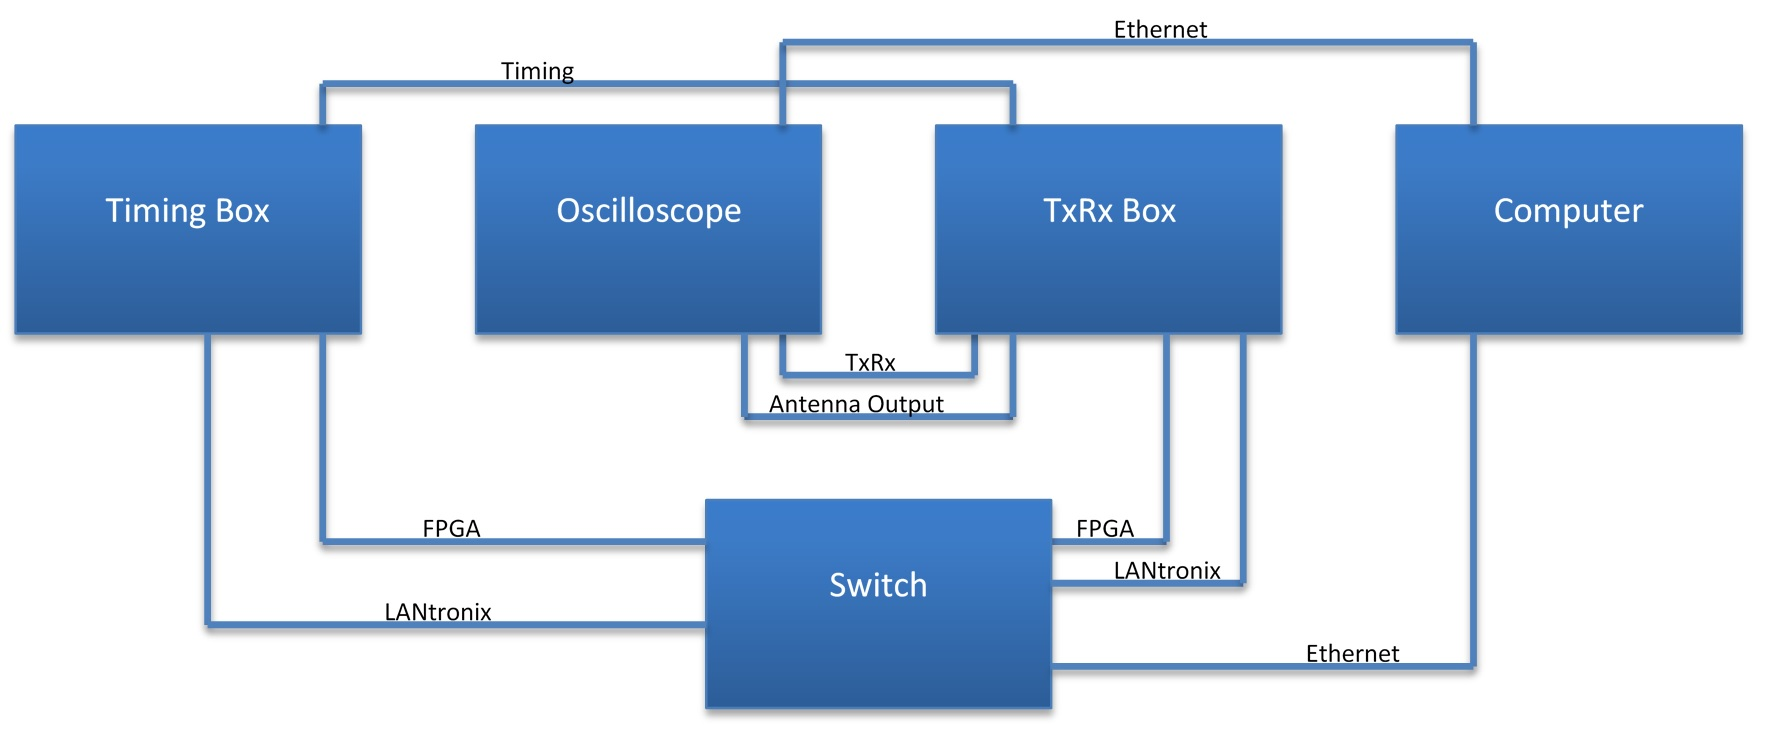
\includegraphics[width=0.7\textwidth]{images/hardware/txrx_setup.jpg}
	\caption{Setup of transceiver box, timing box, oscilloscope and server.}
	\label{fig:hw_txrx_setup}
\end{figure}

\begin{enumerate}
	\item Ensure all cables are plugged in; And the dummy load is connected to the antenna port
	\item On the computer (Joshua) go to /T3/cpart/ [Run command: cd /T3/cpart/]
	\item Run ./sop
	\item Ensure that there are 2 boxes alive (Timing box and Transceiver box being tested)
	\item Enter 1 for transmit test, then 3 to transmit
	\item You should hear the box switching and see the TxRx signal as well as the antenna output (500Vp-p) on the oscilloscope
	\item To stop the test, enter 5 for the receive test, replace the dummy load with AWG set to 9.9MHz @ 1mVp-p
	\item Run ./sop again and enter 0, then 3 to begin
	\item When you switch on the AWG you should see a waveform on the computer with amplitude 30 000 peak-to-peak
	\item To stop the test, enter 5
\end{enumerate}

\subsubsection{Calibration}

\begin{enumerate}
	\item For the calibration, replace the AWG input with the dummy load
	\item Run ./sop and enter 1, then 3 to transmit
	\item Once you hear the switching, press 4 to enter calibration
	\item Enter the box node number you wish to calibrate
	\item Once calibration is complete, do another transmit test and confirm antenna output is 500Vp-p
\end{enumerate}

\clearpage

\subsection{Radar Server and Network}
\label{subsec:hw_network}
A diagram of the server network was shown in the introduction, refer to \figref{intro_hw}. The network and server shouldn't require a lot of maintenance. There is a spare server called Caleb to replace Joshua if it gives any problems. There are several spare parts for the servers as well, which can be found in the VLF store room.
\par
As for the network, some of the LAN cables might get damaged from time to time. In this case they should simply be replaced with spare cables. These are kept in the radar hut too. Make sure that the type of cable is the correct one for the purpose you want to use it for. (The green ones - CAT6 - are especially for the timing cables from the timing box to the transceiver boxes. They should all be of the same length too.)

\clearpage